\documentclass[a4paper,14pt]{extarticle}
\def\source{/home/osabio/tex/templates}
\input{\source/head.tex}
\irodov{3.232}{Магнитостатика}
% Стыдить лжеца, шутить над дураком
% И спорить с женщиной — всё то же,
% Что черпать воду решетом:
% От сих троих избавь нас, боже!..

% М. Ю. Лермонтов.
\usetikzlibrary{decorations.markings}
\usepackage[outline]{contour}
\contourlength{4pt}
\begin{document}

а) поле плоскости
\begin{figure}[H]
    \centering
    \begin{tikzpicture}
    \draw (0,0) -- ++(8,0);

    % \begin{scope}[yshift=2cm]
    %     \lineann[2]{0}{-2}{$a$}
    % \end{scope}


    \draw[->] (2,1.5) -- ++(4,0) node[above,pos=0.5] {$\bf{B}$};
    \draw[<-] (2,-1.5) -- ++(4,0) node[below,pos=0.5] {$\bf{B}$};
    \begin{scope}[
        very thick,decoration={
        markings,
        mark=at position 0.5 with {\arrow{>}}},
        xshift=3cm,
        yshift=-0.5cm,
        ] 


        \draw[postaction={decorate}] (0,0) coordinate (1)-- node[left] {1}(0,1);
        \draw[postaction={decorate}] (0,1) coordinate (2)-- node[above] {2}(2,1);
        \draw[postaction={decorate}] (2,1) coordinate (3)-- node[right] {3}(2,0);
        \draw[postaction={decorate}] (2,0) coordinate (4)-- node[below] {4}(0,0);

        % \draw[dashed] (1) -- (3);
        % \draw[dashed] (2) -- (4);
        % % \draw[dashed] 
        % %     (-4,4) node[above] {$O$}
        % %     -- (0,0) node[anchor=west] {$A$}
        % %     -- (4,-4) node[right] {$O'$};

        % % \draw[dashed] 
        % %     (4,4) node[above] {$B$}
        % %     -- (-4,-4) node[right] {$B'$};            

        % % \draw (135:{sqrt(2)}) node [] {\contour{white}{$\bigotimes$}}  node[above, yshift=0.5em] {$d\vec{B}_1$};
        % \draw (4,2) node [] {\contour{white}{$\bigotimes$}} node[above, yshift=0.5em] {$d\vec{B}_{1,2,3,4}$};

        \draw (4,0.5) node [] {\contour{white}{$\bigotimes$}}  node[above, yshift=0.5em] {$\bf{j}$};
        % \draw (45:2.5) node [] {\contour{white}{$\bigotimes$}} node[above, yshift=0.5em] {$d\vec{B}_2$};     

        % \draw (135+90:{sqrt(2)}) node [] {\contour{white}{$\bigotimes$}}  node[above, yshift=0.5em] {$d\vec{B}_1$};
        % \draw (135+90:2.5) node [] {\contour{white}{$\bigodot$}} node[above, yshift=0.5em] {$d\vec{B}_2$};

        % \draw (45-90:{sqrt(2)}) node [] {\contour{white}{$\bigodot$}}  node[above, yshift=0.5em] {$d\vec{B}_1$};
        % \draw (45-90:2.5) node [] {\contour{white}{$\bigodot$}} node[above, yshift=0.5em] {$d\vec{B}_2$};   

        % \draw (5,0) -- (14,0);          
        % \draw[] (9,-4) -- ++(0,8);          

    \end{scope}    
    \end{tikzpicture}
\end{figure}

Выберем в качестве удобного контура прямоугольник с стороной длины $x$, параллельной плоскости:
\begin{equation}
    \oint\limits_{(L)} \vec{B}d\vec{l}= 
    \int\limits_{(1)} \vec{B}d\vec{l}+
    \int\limits_{(2)} \vec{B}d\vec{l}+
    \int\limits_{(3)} \vec{B}d\vec{l}+
    \int\limits_{(4)} \vec{B}d\vec{l}
\end{equation}
Два участка не дадут вклада, т.к. на них $\vec{B}\perp d \vec{l}$:

\begin{equation}
    \oint\limits_{(L)} \vec{B}d\vec{l}= 
    \int\limits_{(2)} \vec{B}d\vec{l}+
    \int\limits_{(4)} \vec{B}d\vec{l}=
    2B_l\int\limits_{(2)} d\vec{l}=2B_l x
    % =\beta 4\pi J_i
\end{equation}
\begin{equation}
    J_i=jx
\end{equation}

\begin{equation}
    \oint\limits_{(L)} \vec{B}d\vec{l}=
    \beta 4\pi J_i
\end{equation}
\begin{equation}
    2B_l x=\beta 4\pi j x
\end{equation}
\begin{equation}
    B_l=2\beta\pi j
\end{equation}


б) поле параллельных плоскостей
\begin{figure}[H]
    \centering
    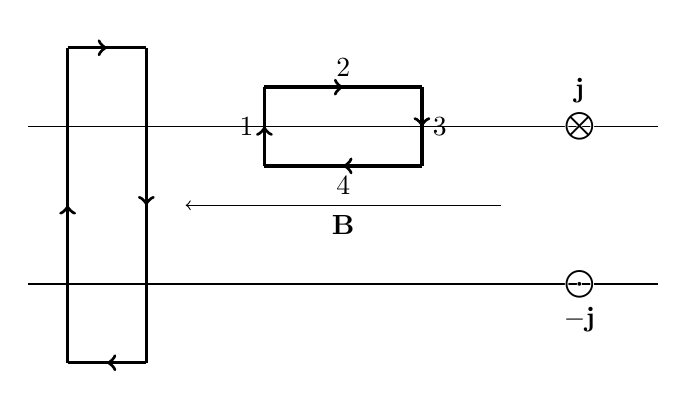
\begin{tikzpicture}
    \draw (0,-1) -- ++(8,0);
    \draw (0,1) -- ++(8,0);

    % \begin{scope}[yshift=2cm]
    %     \lineann[2]{0}{-2}{$a$}
    % \end{scope}


    % \draw[->] (2,2) -- ++(4,0) node[above,pos=0.5] {$\bf{B}$};
    \draw[<-] (2,0) -- ++(4,0) node[below,pos=0.5] {$\bf{B}$};
    \begin{scope}[
        very thick,decoration={
        markings,
        mark=at position 0.5 with {\arrow{>}}},
        xshift=3cm,
        yshift=0.5cm,
        ] 

        \draw[postaction={decorate}] (0,0) coordinate (1)-- node[left] {1}(0,1);
        \draw[postaction={decorate}] (0,1) coordinate (2)-- node[above] {2}(2,1);
        \draw[postaction={decorate}] (2,1) coordinate (3)-- node[right] {3}(2,0);
        \draw[postaction={decorate}] (2,0) coordinate (4)-- node[below] {4}(0,0);   

    \end{scope}  
    \begin{scope}[
        very thick,decoration={
        markings,
        mark=at position 0.5 with {\arrow{>}}},
        xshift=0.5cm,
        yshift=-2cm,
        ] 

        \draw[postaction={decorate}] (0,0) coordinate (1)-- node[left] {}(0,4);
        \draw[postaction={decorate}] (0,4) coordinate (2)-- node[above] {}(1,4);
        \draw[postaction={decorate}] (1,4) coordinate (3)-- node[right] {}(1,0);
        \draw[postaction={decorate}] (1,0) coordinate (4)-- node[below] {}(0,0);   

    \end{scope}       
        \draw (7,1) node [] {\contour{white}{$\bigotimes$}}  node[above, yshift=0.5em] {$\bf{j}$};
        \draw (7,-1) node [] {\contour{white}{$\bigodot$}}  node[below, yshift=-0.5em] {$\bf{-j}$};    
    \end{tikzpicture}
\end{figure}

Вне плоскостей, очевидно, поле будет равно нулю, так как равен нулю суммарный охваченный ток (из теоремы о циркуляции). Можно показать, выбрав контур, захватывающий обе плоскости:

\begin{equation}
    \oint\limits_{(L_1)} \vec{B}d\vec{l}=0 \quad \Rightarrow \quad \vec{B}=\vec{0}
\end{equation}

Между плоскостями найдем поле, выбрав контур $L_2$.

Выберем в качестве удобного контура прямоугольник с стороной длины $x$, параллельной плоскости:
\begin{equation}
    \oint\limits_{(L)} \vec{B}d\vec{l}= 
    \int\limits_{(1)} \vec{B}d\vec{l}+
    \int\limits_{(2)} \vec{B}d\vec{l}+
    \int\limits_{(3)} \vec{B}d\vec{l}+
    \int\limits_{(4)} \vec{B}d\vec{l}
\end{equation}
Два участка не дадут вклада, т.к. на них $\vec{B}\perp d \vec{l}$, а третий (внешний) не даст, так снаружи поля нет:
\begin{equation}
    \oint\limits_{(L)} \vec{B}d\vec{l}= 
    \int\limits_{(4)} \vec{B}d\vec{l}=B_l x
\end{equation}
\begin{equation}
    J_i=jx
\end{equation}
\begin{equation}
    \oint\limits_{(L)} \vec{B}d\vec{l}=
    \beta 4\pi J_i
\end{equation}
\begin{equation}
    B_l x=\beta 4\pi j x
\end{equation}
\begin{equation}
    B_l=4\beta\pi j
\end{equation}


\end{document}